\chapter{The Land Surface Climate in the Regional Arctic System Model - Supplemental Materials}
\label{chap:land_surface_sup}

This appendix includes the supplemental materials from chapter \ref{chap:land_surface}.
This material has been published in its current form in the \textit{Journal of Climate}.
\textcopyright American Meteorological Society.
Used with permission.

\bibentry{Hamman_2016a}.

\section{Figures}

\begin{figure}
    \centering
    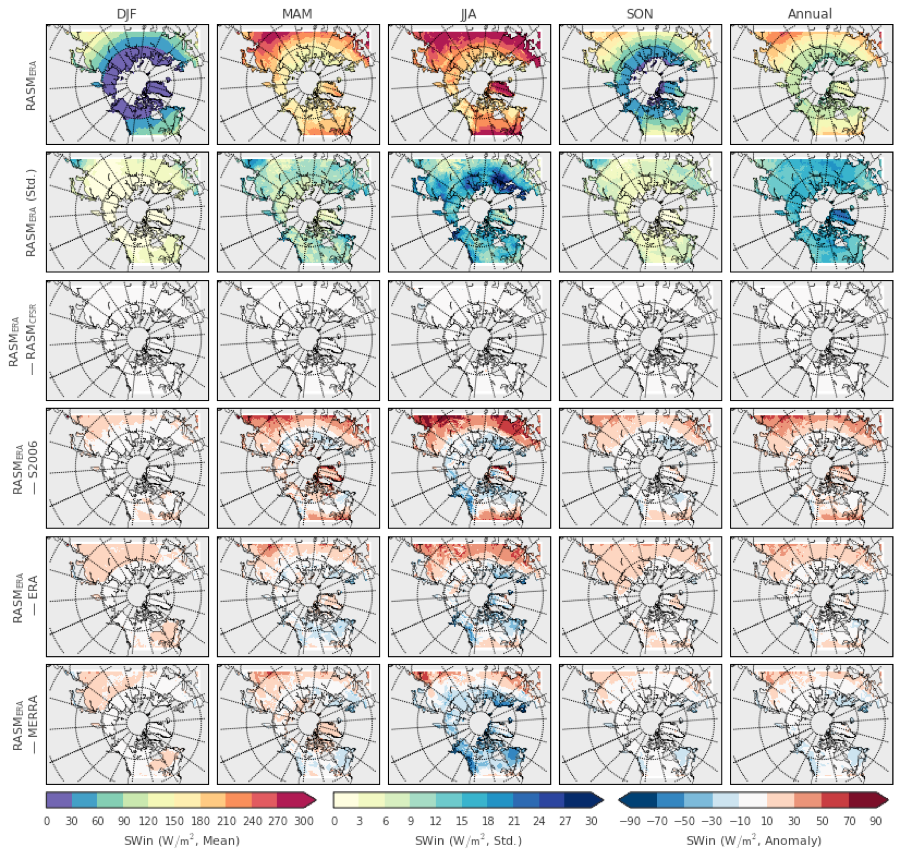
\includegraphics[width=16cm,keepaspectratio]{ch3_S1}
    \caption{Seasonal and annual average downward shortwave radiation (SWin).
    Time period: Sep. 1989 – Aug. 2014.}
\end{figure}

\begin{figure}
    \centering
    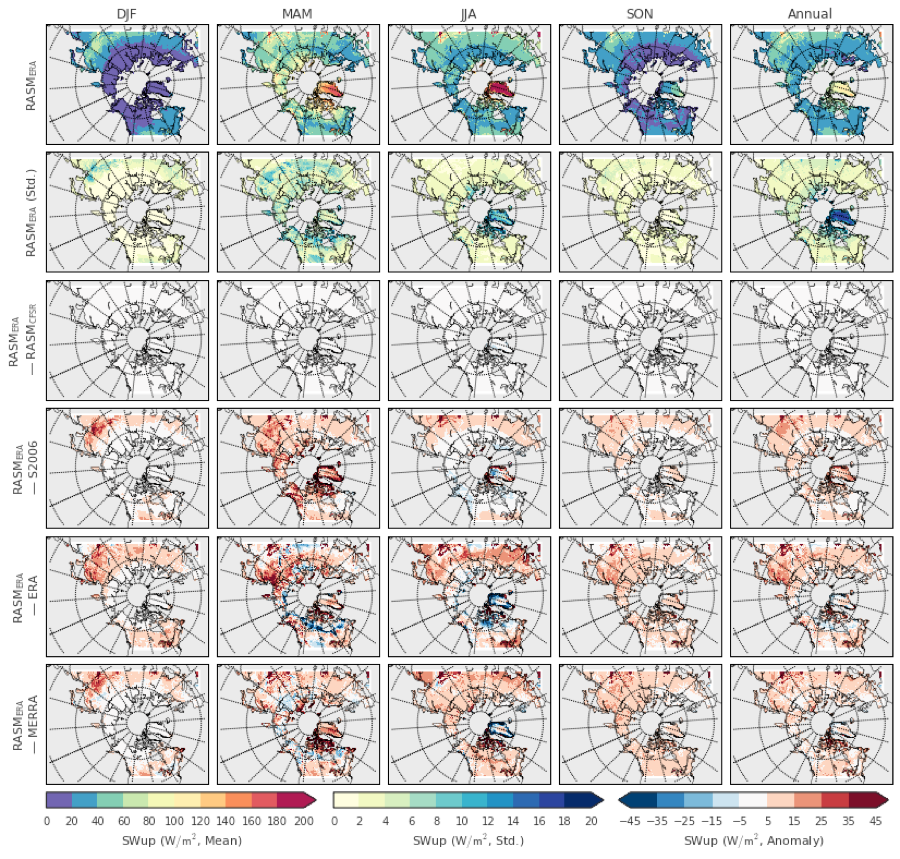
\includegraphics[width=16cm,keepaspectratio]{ch3_S2}
    \caption{Seasonal and annual average upward (reflected) shortwave radiation (SWup).
    Time period: Sep. 1989 – Aug. 2014.}
\end{figure}

\begin{figure}
    \centering
    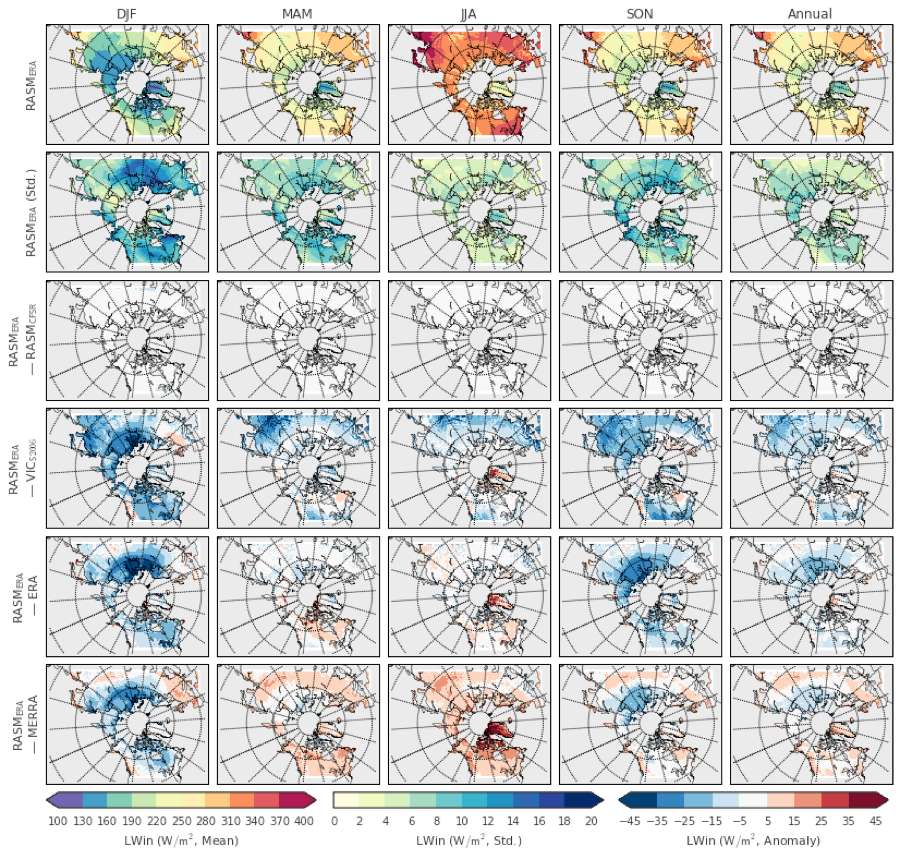
\includegraphics[width=16cm,keepaspectratio]{ch3_S3}
    \caption{Seasonal and annual average downward longwave radiation (LWin).
    Time period: Sep. 1989 – Aug. 2014.}
\end{figure}

\begin{figure}
    \centering
    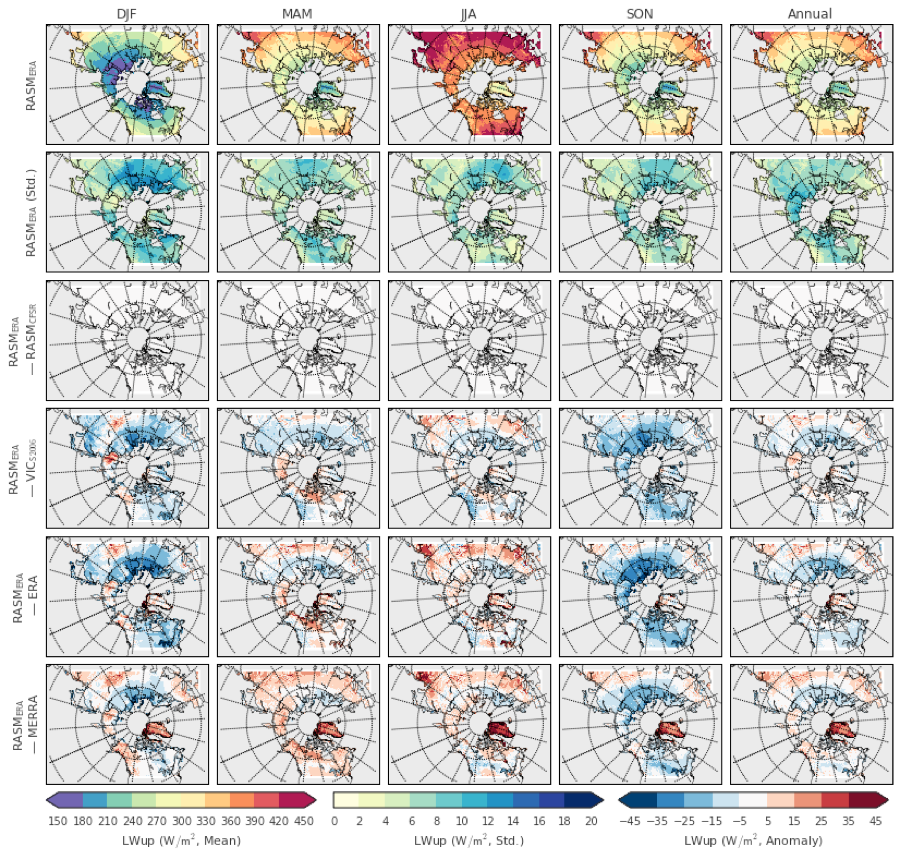
\includegraphics[width=16cm,keepaspectratio]{ch3_S4}
    \caption{Seasonal and annual average upward longwave radiation (LWup).
    Time period: Sep. 1989 – Aug. 2014.}
\end{figure}

\begin{figure}
    \centering
    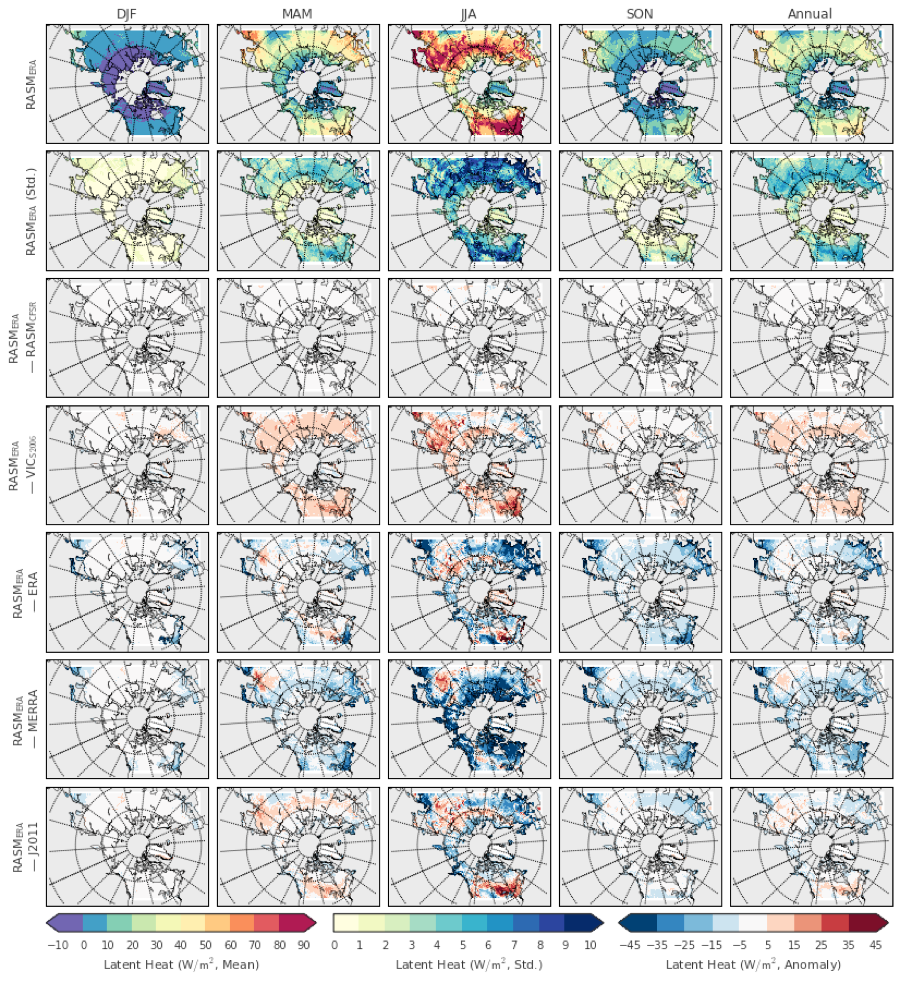
\includegraphics[width=16cm,keepaspectratio]{ch3_S5}
    \caption{Seasonal and annual average latent heat flux (LE).
    Time period: Sep. 1989 – Aug. 2014.}
\end{figure}

\begin{figure}
    \centering
    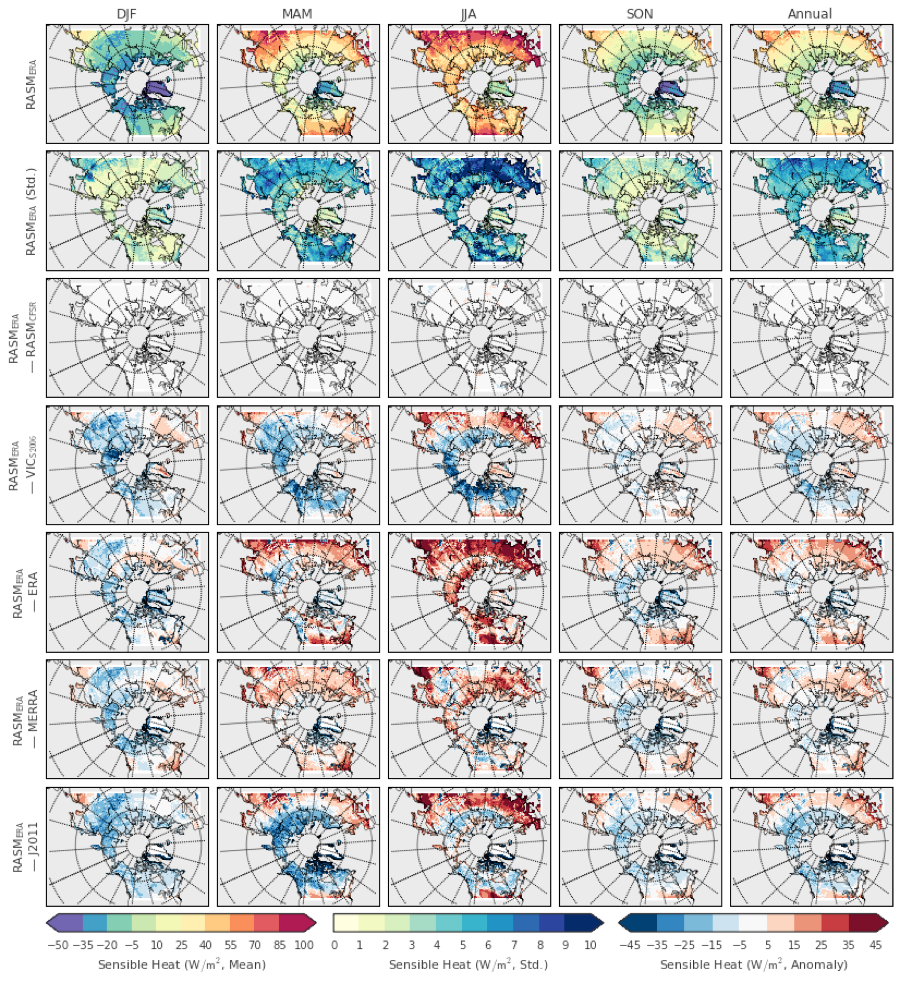
\includegraphics[width=16cm,keepaspectratio]{ch3_S6}
    \caption{Seasonal and annual average sensible heat flux (H).
    Time period: Sep. 1989 – Aug. 2014.}
\end{figure}

\begin{figure}
    \centering
    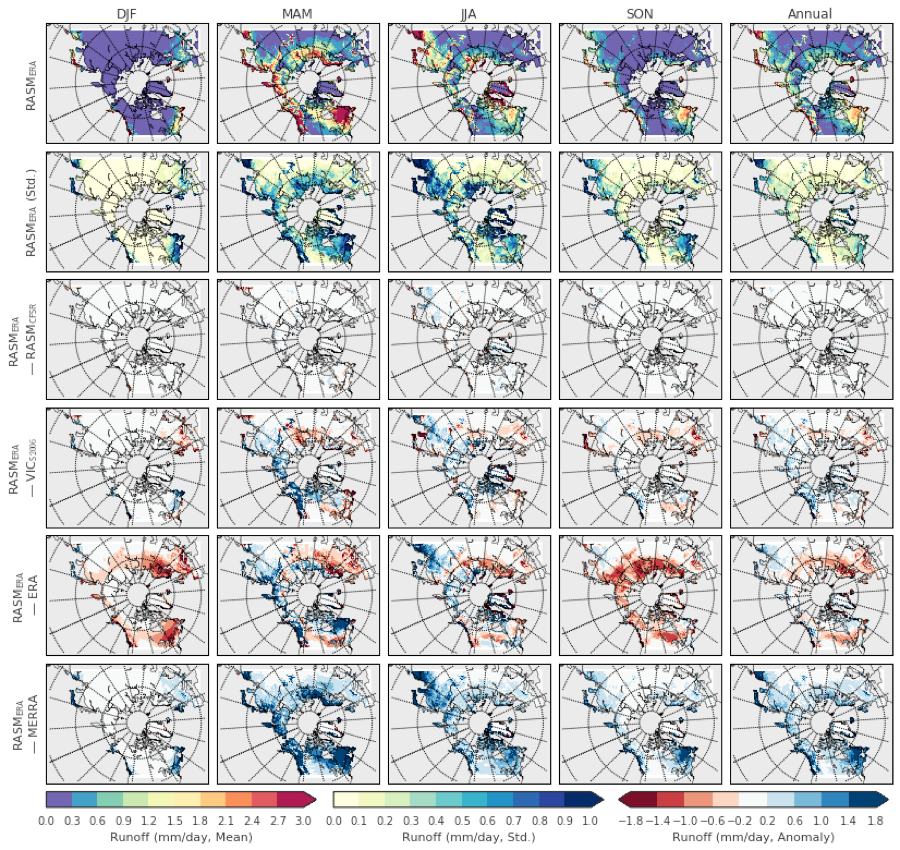
\includegraphics[width=16cm,keepaspectratio]{ch3_S7}
    \caption{Seasonal and annual runoff (Q).
    Time period: Sep. 1989 – Aug. 2014.}
\end{figure}

\begin{figure}
    \centering
    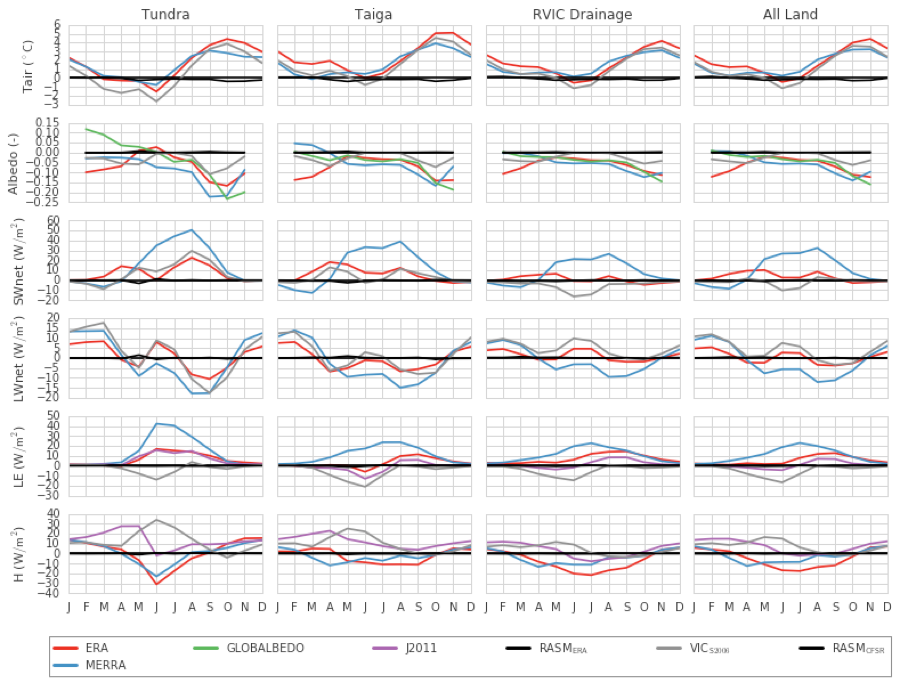
\includegraphics[width=16cm,keepaspectratio]{ch3_S8}
    \caption{Difference (RASM – X) in average seasonal cycles of surface air temperature (Tair), albedo, net shortwave radiation (SWnet), net longwave radiation (LWnet), latent heat flux (LE), and sensible heat flux (H) for tundra, taiga, RVIC drainage, and full model domain.
    Time period: 1990-2014.}
\end{figure}

\begin{figure}
    \centering
    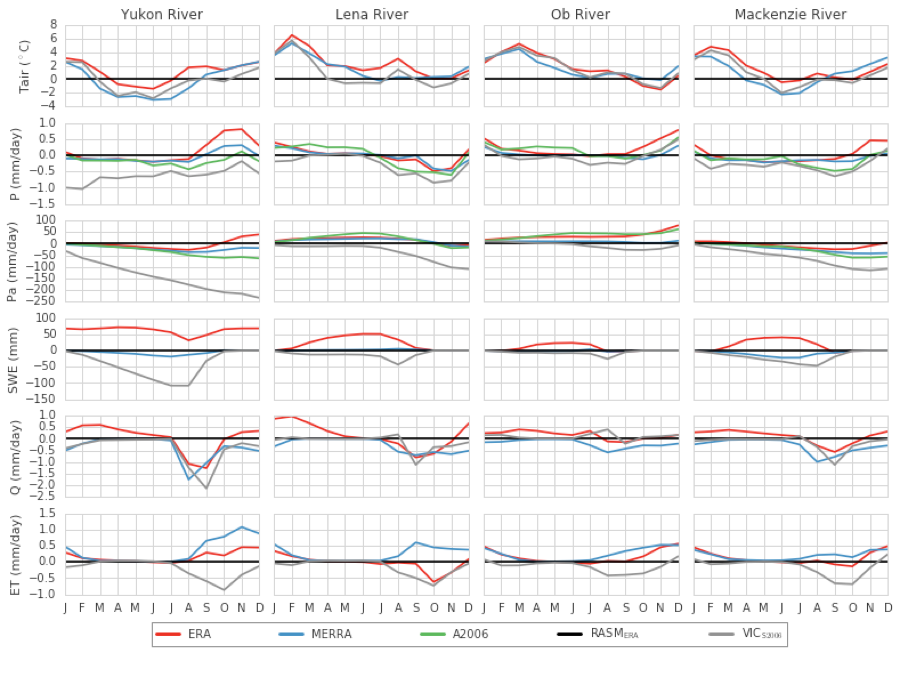
\includegraphics[width=16cm,keepaspectratio]{ch3_S9}
    \caption{Difference (RASM – X) in average seasonal cycles of surface air temperature (Tair), precipitation (P), accumulated precipitation (Pa), runoff (Q), evapotranspiration (ET) and snow water equivalent (SWQ) for four of the largest river basins in the RASM domain.
    Time period: 1990-2014.}
\end{figure}

\clearpage
\section{Tables}

\begin{table}[]
\centering
\caption{Summary of land surface parameters used by the VIC model.}
\label{table:s1}
\resizebox{\textwidth}{!}{
\begin{tabular}{ll}
\hline
\textbf{Parameters}                                                        & \textbf{Values or Source}           \\ \hline
Physical parameters (soil density, saturated hydraulic conductivity, etc.) & \citet{Sheffield_2006}              \\
Calibratable parameters (baseflow, infiltration, etc.)                     & \citet{Sheffield_2006},             \\
                                                                           & Inside Permafrost Region: Dsmax ≈ 0 \\
Soil depths                                                                & 0.1 m / 0.9 m / 2.5 m               \\
Vegetation resistance parameters                                           & \citet{Nijssen_1997}                \\
Canopy Layers                                                              & 1                                   \\
Land Surface Emissivity                                                    & 0.97                                \\
Bare Surface Albedo                                                        & 0.55                                \\
Fresh Snow Albedo                                                          & 0.85                                \\
Maximum Snow Covered Vegetation Albedo                                     & \citet{Barlage_2005}                \\ \hline
\end{tabular}
}
\end{table}

\begin{table}[]
\centering
\caption{Summary of land-atmosphere coupled variables in RASM.}
\label{table:s2}
 \resizebox{\textwidth}{!}{
\begin{tabular}{ll}
\hline
Coupled Fields – Coupler to Land (units)                   & Coupled Fields – Land to Coupler (units)            \\ \hline
Height of atmosphere lowest model level (m)                & Liquid runoff flux (kg m-1 s-1)                     \\
Zonal wind at atmosphere lowest model level (m/s)          & Surface temperature (K)                             \\
Meridional wind at atmosphere lowest model level (m/s)     & 2-m reference air temperature (K)                   \\
Potential temperate at atmosphere lowest model level (K)   & 2-m reference specific humidity (-)                 \\
Specific humidity at atmosphere lowest model level (-)     & Direct, visible surface albedo (-)                  \\
Atmospheric pressure at atmosphere lowest model level (Pa) & Direct, near-infrared surface albedo (-)            \\
Temperature at atmosphere lowest model level (K)           & Diffuse, visible surface albedo (-)                 \\
Downwelling longwave radiation flux (W m-2)                & Diffuse, near-infrared surface albedo (-)           \\
Direct near-infrared shortwave radiation flux (W m-2)      & Snow height (m)                                     \\
Direct visible shortwave radiation flux (W m-2)            & Log Z0 (-)                                          \\
Diffuse near-infrared shortwave radiation flux (W m-2)     & Zonal wind stress (Pa)                              \\
Diffuse visible shortwave radiation flux (W m-2)           & Meridional wind stress (Pa)                         \\
Convective liquid precipitation flux (kg m-1 s-1)          & Latent heat flux (W m-2)                            \\
Large scale liquid precipitation flux (kg m-1 s-1)         & Sensible heat flux (W m-2)                          \\
Convective frozen precipitation flux (kg m-1 s-1)          & Upwelling longwave radiation flux (W m-2)           \\
Large scale frozen precipitation flux (kg m-1 s-1)         & Evaporation flux (kg m-1 s-1)                       \\
                                                           & Net shortwave radiation flux at the surface (W m-2) \\ \hline
\end{tabular}
}
\end{table}

\begin{landscape}
\begin{table}[]
\centering
\caption{Summary of comparison datasets used to compare to RASM land surface output.}
\label{table:s3}
\resizebox{22cm}{!}{
\begin{tabular}{p{3in}lllll}
\hline
\textbf{Dataset}                                                                 & \textbf{Label} & \textbf{Data Type}              & \textbf{Spatial Coverage}        & \textbf{Temporal Coverage} & \textbf{Reference}           \\ \hline
ECMWF’s ERA-interim Reanalysis                                                   & ERA            & Reanalysis                      & Global - T255 (approx. 80 km)    & 1979-present               & \citet{Dee_2011}             \\
                                                                                 &                &                                 &                                  & 3-hourly                   &                              \\
NASA’s Modern-Era Retrospective Analysis for Research and Applications           & MERRA          & Reanalysis                      & Global – 1/2$^{\circ}$ × 2/3 $^{\circ}$            & 1979-present               & \citet{Rienecker_2011}       \\
                                                                                 &                &                                 &                                  & 3-hourly                   &                              \\
Global Meteorological Forcing Dataset for land surface modeling                  & S2006          & Bias Corrected Reanalysis       & Global - 1$^{\circ}$                      & 1948-2010, 3-hourly        & \citet{Sheffield_2006}       \\
Global 1/2$^{\circ}$ Gridded Meteorological VIC Forcing Data Set                          & A2006          & Bias Corrected Reanalysis       & Global Land – 0.5$^{\circ}$               & 1948-2007, daily           & \citet{Adam_2006}            \\
Northern Hemisphere EASE-Grid 2.0 Weekly Snow Cover Extent, Version 4            & NSIDC          & Remote Sensing                  & Northern Hemisphere Land - 25 km & 1966-2014, weekly          & \citet{Brodzik_2013}         \\
ESA High Resolution Global Albedo Data Set                                       & GlobAlbedo     & Remote Sensing                  & Global Land – 1km                & 1998-2011, monthly         & \citet{Muller_2012}          \\
Empirically Upscaled Gridded FLUXNET Data Set                                    & J2011          & Reanalysis / Observations       & Global Land – 0.5$^{\circ}$               & 1982-2011                  & \citet{Jung_2011}            \\
Regional, Electronic, Hydrographic Data Network For the Arctic Region, Version 4 & R-ArcticNET    & In-situ Streamflow Observations & Pan-arctic, 3754 gauges          & 1960-2001,                 & \citet{Lammers_2001}         \\
                                                                                 &                &                                 &                                  & monthly                    &                              \\
AmeriFlux: Regional flux tower network database                                  & AmeriFlux      & In-situ Flux Tower Observations & Global, 2 stations used          & 1994-1995 (used)           &                              \\ \hline
\end{tabular}
}
\end{table}
\end{landscape}

\begin{table}[]
\centering
\caption{Variables analyzed and datasets each variable is compared to.}
\label{table:s4}
\resizebox{12cm}{!}{

\begin{tabular}{lll}
\hline
\textbf{Variable}     & \textbf{Abbreviation} & \textbf{Compared to:}        \\ \hline
2m Air Temperature    & Tair                  & ERA, MERRA, S2006, AmeriFlux \\
Surface Albedo        & Albedo                & ERA, MERRA, GlobAlbedo       \\
Shortwave Radiation   & SW\{in,up,net\}       & ERA, MERRA, S2006            \\
Longwave Radiation    & LW\{in,up,net\}       & ERA, MERRA, S2006            \\
Latent Heat           & LH                    & ERA, MERRA, J2011, AmeriFlux \\
Sensible Heat         & H                     & ERA, MERRA, J2011, AmeriFlux \\
Total Precipitation   & P                     & ERA, MERRA, S2006, A2006     \\
Total Runoff          & Q                     & ERA, MERRA, R-ArcticNET      \\
Evapotranspiration    & ET                    & ERA, MERRA                   \\
Snow Water Equivalent & SWQ                   & ERA, MERRA                   \\
Snow Cover Extent     & SCE                   & ERA, MERRA, NSIDC            \\ \hline
\end{tabular}
}
\end{table}

\begin{table}
\centering
\caption{Seasonal and annual averages for selected variables for the tundra and taiga bioregions. Time period 1990-2014.}
\label{table:s5}
\resizebox{10cm}{!}{
\begin{tabular}{lllllllllll}
Taiga                                          &                              &        &        &        & Tundra &        &        &        &        &        \\
                                               & DJF                          & MAM    & JJA    & SON    & Annual & DJF    & MAM    & JJA    & SON    & Annual \\
Albedo (-)                                     &                              &        &        &        &        &        &        &        &        &        \\
ERA                                            & 0.3                          & 0.26   & 0.15   & 0.19   & 0.2    & 0.53   & 0.54   & 0.29   & 0.33   & 0.4    \\
MERRA                                          & 0.47                         & 0.3    & 0.12   & 0.16   & 0.2    & 0.55   & 0.51   & 0.2    & 0.27   & 0.33   \\
$RASM_{CFSR}$                                       & 0.44                         & 0.32   & 0.18   & 0.3    & 0.27   & 0.62   & 0.57   & 0.31   & 0.54   & 0.45   \\
$RASM_{ERA}$                                        & 0.44                         & 0.32   & 0.18   & 0.3    & 0.26   & 0.62   & 0.57   & 0.3    & 0.54   & 0.44   \\
Bowen Ratio, B (-)                             &                              &        &        &        &        &        &        &        &        &        \\
2.82                                           & 1.2                          & 0.52   & -0.22  & 0.42   & 2.98   & 1.52   & 0.28   & -1.57  & -0.17  & 2.82   \\
-48.06                                         & 0.6                          & 0.51   & -0.06  & 0.37   & 54.5   & 0.46   & 0.67   & -1.33  & 0.36   & -48.06 \\
-9                                             & 1.14                         & 0.76   & -1     & 0.53   & 108.32 & -0.08  & 1.44   & 14.62  & -1.59  & -9     \\
14.27                                          & 1.13                         & 0.76   & -0.44  & 0.54   & 18.6   & -1.15  & 1.55   & 1.81   & -0.94  & 14.27  \\
Evapotranspiration, ET (mm/day)                &                              &        &        &        &        &        &        &        &        &        \\
ERA                                            & 0.06                         & 0.82   & 2.35   & 0.59   & 0.95   & 0.07   & 0.33   & 1.33   & 0.3    & 0.51   \\
MERRA                                          & 0.08                         & 1.14   & 3.09   & 0.69   & 1.25   & 0      & 0.48   & 2.15   & 0.27   & 0.72   \\
$RASM_{CFSR}$                                       & 0.01                         & 0.82   & 2.32   & 0.32   & 0.86   & -0.02  & 0.29   & 1.01   & 0.08   & 0.34   \\
$RASM_{ERA}$                                        & 0.01                         & 0.84   & 2.32   & 0.32   & 0.88   & -0.02  & 0.29   & 1.02   & 0.08   & 0.35   \\
Latent Heat Flux, LE (W/m2)                    &                              &        &        &        &        &        &        &        &        &        \\
ERA                                            & 2.08                         & 24.72  & 67.81  & 17.41  & 27.95  & 2.01   & 10.42  & 38.49  & 8.81   & 14.9   \\
MERRA                                          & 2.46                         & 33.94  & 87.85  & 19.74  & 35.92  & 0.05   & 14.86  & 61.26  & 7.82   & 20.92  \\
$RASM_{CFSR}$                                       & 0.44                         & 24.41  & 66.11  & 9.31   & 24.95  & -0.76  & 9.04   & 29.07  & 2.27   & 9.85   \\
$RASM_{ERA}$                                        & 0.47                         & 24.91  & 66.13  & 9.41   & 25.41  & -0.76  & 9.1    & 29.3   & 2.37   & 10.08  \\
Net Longwave Radiation Flux, LWnet (W/m2)      &                              &        &        &        &        &        &        &        &        &        \\
ERA                                            & -32.74                       & -56.8  & -58.39 & -40.51 & -47.07 & -31.08 & -43.81 & -45.65 & -35.25 & -38.92 \\
MERRA                                          & -28.91                       & -54.3  & -65.93 & -44.15 & -48.32 & -21.81 & -42.68 & -60.67 & -33.28 & -39.59 \\
$RASM_{CFSR}$                                       & -39.52                       & -53.29 & -55.62 & -38.71 & -46.72 & -38.18 & -47.65 & -48.93 & -33.59 & -42.01 \\
$RASM_{ERA}$                                        & -39.57                       & -53.89 & -55.72 & -38.55 & -46.99 & -38.21 & -48.03 & -48.86 & -33.45 & -42.18 \\
P-E (mm/day)                                   &                              &        &        &        &        &        &        &        &        &        \\
ERA                                            & 0.9                          & 0.49   & 0.26   & 1.25   & 0.73   & 0.73   & 0.58   & 0.52   & 1.13   & 0.74   \\
MERRA                                          & 0.86                         & 0.18   & -0.73  & 1.06   & 0.35   & 0.77   & 0.43   & -0.39  & 1.1    & 0.48   \\
$RASM_{CFSR}$                                       & 0.97                         & 0.62   & 0.04   & 1.31   & 0.74   & 0.84   & 0.74   & 0.7    & 1.33   & 0.91   \\
$RASM_{ERA}$                                        & 0.96                         & 0.6    & 0.07   & 1.32   & 0.73   & 0.83   & 0.73   & 0.73   & 1.36   & 0.91   \\
Precipitation, P (mm/day)                      &                              &        &        &        &        &        &        &        &        &        \\
ERA                                            & 0.96                         & 1.31   & 2.61   & 1.85   & 1.68   & 0.8    & 0.91   & 1.85   & 1.43   & 1.25   \\
MERRA                                          & 0.94                         & 1.33   & 2.36   & 1.74   & 1.59   & 0.83   & 0.94   & 1.8    & 1.42   & 1.25   \\
$RASM_{CFSR}$                                       & 0.98                         & 1.44   & 2.36   & 1.63   & 1.6    & 0.82   & 1.02   & 1.72   & 1.41   & 1.24   \\
$RASM_{ERA}$                                        & 0.97                         & 1.44   & 2.39   & 1.64   & 1.61   & 0.81   & 1.02   & 1.75   & 1.44   & 1.26   \\
Total Runoff, Q (mm/day)                       &                              &        &        &        &        &        &        &        &        &        \\
ERA                                            & 0.55                         & 1.18   & 0.92   & 1.07   & 0.93   & 0.21   & 0.87   & 1.38   & 0.9    & 0.84   \\
MERRA                                          & 0.1                          & 0.76   & 0.31   & 0.18   & 0.34   & 0.09   & 0.72   & 0.83   & 0.22   & 0.46   \\
$RASM_{CFSR}$                                       & 0.13                         & 1.51   & 0.8    & 0.47   & 0.72   & 0.09   & 1.49   & 1.55   & 0.43   & 0.89   \\
$RASM_{ERA}$                                        & 0.13                         & 1.51   & 0.8    & 0.47   & 0.73   & 0.09   & 1.52   & 1.54   & 0.45   & 0.91   \\
Runoff Ratio, Q/P (-)                          &                              &        &        &        &        &        &        &        &        &        \\
ERA                                            & 0.52                         & 0.93   & 0.33   & 0.58   & 0.53   & 0.18   & 0.95   & 0.88   & 0.62   & 0.68   \\
MERRA                                          & 0.06                         & 0.49   & 0.11   & 0.07   & 0.17   & 0.04   & 0.59   & 0.42   & 0.1    & 0.29   \\
$RASM_{CFSR}$                                       & 0.06                         & 0.98   & 0.31   & 0.22   & 0.4    & 0.03   & 1.38   & 0.93   & 0.23   & 0.69   \\
$RASM_{ERA}$                                        & 0.07                         & 0.98   & 0.31   & 0.22   & 0.4    & 0.03   & 1.42   & 0.91   & 0.23   & 0.7    \\
                                               & Sensible Heat Flux, H (W/m2) &        &        &        &        &        &        &        &        &        \\
ERA                                            & -13.76                       & 29.02  & 34.23  & -2.46  & 11.67  & -10.3  & 5.79   & 21.67  & -1.26  & 3.95   \\
MERRA                                          & -11.78                       & 20.58  & 40.64  & -1.28  & 11.97  & -12.27 & 7.06   & 36.81  & -4.92  & 6.61   \\
$RASM_{CFSR}$                                       & -17.72                       & 28.49  & 45.2   & -0.82  & 13.68  & -29.25 & 2.65   & 41.17  & -15.93 & -0.45  \\
$RASM_{ERA}$                                        & -17.5                        & 28.76  & 45.39  & -0.84  & 14.16  & -29.2  & 2.92   & 41.05  & -15.93 & -0.09  \\
Downward Shortwave Radiation Flux, SWin (W/m2) &                              &        &        &        &        &        &        &        &        &        \\
ERA                                            & 25.37                        & 175.49 & 209.65 & 57.52  & 116.63 & 8.99   & 159.39 & 198.4  & 34.99  & 100.02 \\
MERRA                                          & 26.22                        & 172.98 & 231.39 & 67.5   & 124.22 & 8.89   & 150.52 & 214.45 & 40.59  & 103.25 \\
$RASM_{CFSR}$                                       & 33.22                        & 169.3  & 206.52 & 65.92  & 118.34 & 11.57  & 158.58 & 186.52 & 39.69  & 98.62  \\
$RASM_{ERA}$                                        & 33.63                        & 170.28 & 206.83 & 65.7   & 119.72 & 11.71  & 159.17 & 185.69 & 39.36  & 99.62  \\
Net Shortwave Radiation Flux, SWnet (W/m2)     &                              &        &        &        &        &        &        &        &        &        \\
ERA                                            & 18.05                        & 129.79 & 178.98 & 46.96  & 93.15  & 4.73   & 74.21  & 138.21 & 24.08  & 60.08  \\
MERRA                                          & 14.13                        & 121.24 & 204.8  & 56.8   & 99.03  & 3.92   & 71.68  & 174.74 & 30.3   & 69.94  \\
$RASM_{CFSR}$                                       & 19.12                        & 114.79 & 169.92 & 46.63  & 87.31  & 4.74   & 67.21  & 128.81 & 19.1   & 54.68  \\
$RASM_{ERA}$                                        & 19.38                        & 116.15 & 170.2  & 46.59  & 88.57  & 4.8    & 68.12  & 128.74 & 19.14  & 55.57  \\
Upward Shortwave Radiation Flux, SWup (W/m2)   &                              &        &        &        &        &        &        &        &        &        \\
ERA                                            & 7.32                         & 45.7   & 30.67  & 10.56  & 23.48  & 4.26   & 85.18  & 60.19  & 10.92  & 39.94  \\
MERRA                                          & 11.71                        & 50.68  & 26.62  & 10.64  & 24.82  & 4.79   & 75.79  & 44.91  & 10.25  & 33.79  \\
$RASM_{CFSR}$                                       & 14.11                        & 54.5   & 36.61  & 19.29  & 31.03  & 6.83   & 91.37  & 57.7   & 20.59  & 43.94  \\
$RASM_{ERA}$                                        & 14.25                        & 54.13  & 36.63  & 19.1   & 31.15  & 6.91   & 91.05  & 56.95  & 20.22  & 44.05  \\
Surface Air Temperature, Tair (C)              &                              &        &        &        &        &        &        &        &        &        \\
ERA                                            & -20.36                       & -2.88  & 14.07  & -2.36  & -2.86  & -25.58 & -12.62 & 7.6    & -8.17  & -9.66  \\
MERRA                                          & -21.59                       & -4     & 14.55  & -3.36  & -3.58  & -24.8  & -11.2  & 8.36   & -8.76  & -9.08  \\
$RASM_{CFSR}$                                       & -23.28                       & -4.46  & 13.12  & -7.15  & -5.44  & -28.49 & -12.08 & 7.21   & -12.84 & -11.54 \\
$RASM_{ERA}$                                        & -23.39                       & -4.28  & 13.3   & -6.9   & -5.21  & -28.39 & -11.9  & 7.38   & -12.45 & -11.24
\end{tabular}
}
\end{table}
